\documentclass[11pt,a4paper]{article}

\usepackage[utf8]{inputenc}
\usepackage[T1]{fontenc}
\usepackage{lmodern}
\usepackage{amsmath,amssymb}
\usepackage{algorithm}
\usepackage{algpseudocode}
\usepackage{booktabs}
\usepackage[authoryear,round]{natbib}
\usepackage{hyperref}
\usepackage{listings}
\usepackage{xcolor}
\usepackage[margin=2.5cm]{geometry}
\usepackage{enumitem}
\usepackage{graphicx}
\usepackage{tikz}
\usetikzlibrary{arrows.meta,positioning,shapes.geometric,calc,fit,backgrounds}
\setlength{\parskip}{0.4em}
\setlength{\parindent}{0em}

\hypersetup{
    colorlinks=true,
    linkcolor=blue!60!black,
    citecolor=blue!60!black,
    urlcolor=blue!60!black
}

\definecolor{codebg}{HTML}{F5F5F5}
\definecolor{teal}{HTML}{0D9488}
\definecolor{violet}{HTML}{A78BFA}
\definecolor{amber}{HTML}{FBBF24}

\tikzset{
    diag title/.style={font=\sffamily\small\bfseries},
    diag box/.style={
        draw=black!75,
        rounded corners=1.5pt,
        fill=gray!4,
        minimum height=0.82cm,
        minimum width=2.5cm,
        align=center,
        font=\sffamily\small,
        inner sep=4pt
    },
    diag data/.style={diag box, rounded corners=0.5pt, fill=gray!8},
    diag ai/.style={diag box, rounded corners=4pt, fill=gray!11},
    diag det/.style={diag box, rounded corners=0.5pt, fill=gray!12, line width=1.0pt},
    diag out/.style={diag box, fill=white},
    diag header/.style={diag box, fill=gray!10, font=\ttfamily\small},
    diag decision/.style={
        draw=black!75,
        diamond,
        aspect=2.35,
        fill=white,
        inner sep=2pt,
        align=center,
        font=\sffamily\scriptsize
    },
    diag terminal/.style={
        draw=black!75,
        rounded corners=1.5pt,
        fill=gray!2,
        minimum height=0.7cm,
        minimum width=1.95cm,
        align=center,
        font=\sffamily\scriptsize\bfseries,
        inner sep=4pt
    },
    diag code/.style={font=\ttfamily\scriptsize, align=left},
    diag note/.style={font=\sffamily\scriptsize, text=black!70, align=center},
    diag label/.style={font=\sffamily\scriptsize, text=black!60},
    diag arrow/.style={-{Stealth[length=4pt]}, semithick, draw=black!70},
    diag feedback/.style={-{Stealth[length=4pt]}, dashed, semithick, draw=black!60}
}

\lstset{
    upquote=true,
    basicstyle=\small\ttfamily,
    backgroundcolor=\color{codebg},
    frame=single,
    framerule=0.5pt,
    rulecolor=\color{gray!30},
    breaklines=true,
    columns=flexible,
    keepspaces=true,
    tabsize=2
}


\title{\textbf{ProveML: Inline Claim Markup for Deterministic Verification of AI-Generated Text}}
\author{Shane Deconinck\\\small{abovebeyond.ai}\\\small{\texttt{hello@shanedeconinck.be}}}
\date{August 2026}

\begin{document}

\maketitle

\begin{abstract}
Organizations are deploying LLMs in consequential settings under regulatory pressure, but most generated text carries no machine-checkable link between individual claims and the underlying data. Each generation of models produces more fluent output, but none can reliably signal its own uncertainty.

\vspace{0.4em}
We present ProveML, a lightweight Markdown extension that places AI-generated claims inside a verifiable boundary. Three inline constructs declare entities, link facts to a data source, and check qualitative judgments against composable, pre-declared thresholds:

\vspace{0.3em}
{\small\texttt{@[student:42]\{Alex\} scored \%[passRate]\{5\}\% and is ?[r: IS\_AT\_RISK]\{at risk\}.}}

\vspace{0.3em}
\noindent Verification is deterministic --- string equality and arithmetic against a flat key-value store, with no model in the loop --- so it is instant (under 0.2\,ms per claim), explainable, and can sit inside a generation loop that feeds each error back to the model; the same verifier can audit text it did not generate.

\vspace{0.4em}
\textbf{What it requires, costs and cannot do.} ProveML applies where the claims are backed by an addressable structured source: without a fact store there is nothing to resolve against. Marked-up responses ran 52--60\% longer in characters than the same text without markup, and three quarters of queries needed no correction pass while a quarter exhausted all three. Exact string equality forbids rounded prose --- a verified sentence must say \texttt{391035000000}, not ``\$391 billion'' --- derived values with no path in the store cannot be bound, and the threshold construct, while specified and tested, was never produced by a model in our benchmark runs.

\vspace{0.4em}
We evaluate across four models (3.8B to API-scale) and two domains --- a generated educational benchmark and real SEC EDGAR filings --- with a reimplemented SymGen baseline and ablations on prompt language and context size. Three findings carry the paper. Whether a model produces verifiable markup at all depends on the shape of the request more than on the size of the model. Verification rate alone overstates how much of a report has been checked, so we pair it with a markup-coverage metric and show the two can diverge widely at identical rates. And both ProveML and substitution fail on addressability, but differently: substitution leaves a hole in the sentence, ProveML leaves a flagged claim carrying the value that was expected instead. The specification, verifier, reference implementation, benchmarks and all run artifacts are published.
\end{abstract}

\noindent\textbf{Keywords:} AI verification, markup language, deterministic verification, structured data, threshold registry, hallucination detection, inline tagging


\section{Introduction}

Large Language Models (LLMs) produce fluent, contextually appropriate text that is increasingly difficult to distinguish from human-authored content. This fluency, however, coexists with a fundamental reliability problem: \textbf{LLMs hallucinate}. They generate text that is plausible but factually incorrect, including fabricated citations, invented statistics, and misattributed claims.

In one line: \textbf{ProveML is iXBRL for AI-generated text.} Financial reporting solved a version of this problem two decades ago by embedding machine-readable tags in human-readable filings, so a regulator can audit a number without reading the prose around it \citep{ixbrl}. ProveML applies that idea where the author is a model rather than a person, and adds what that setting needs: entity scoping, so a value is bound to the record it describes, and a threshold registry, so a qualitative judgment is a declared predicate rather than a choice of adjective.

\begin{figure}[h]
\centering
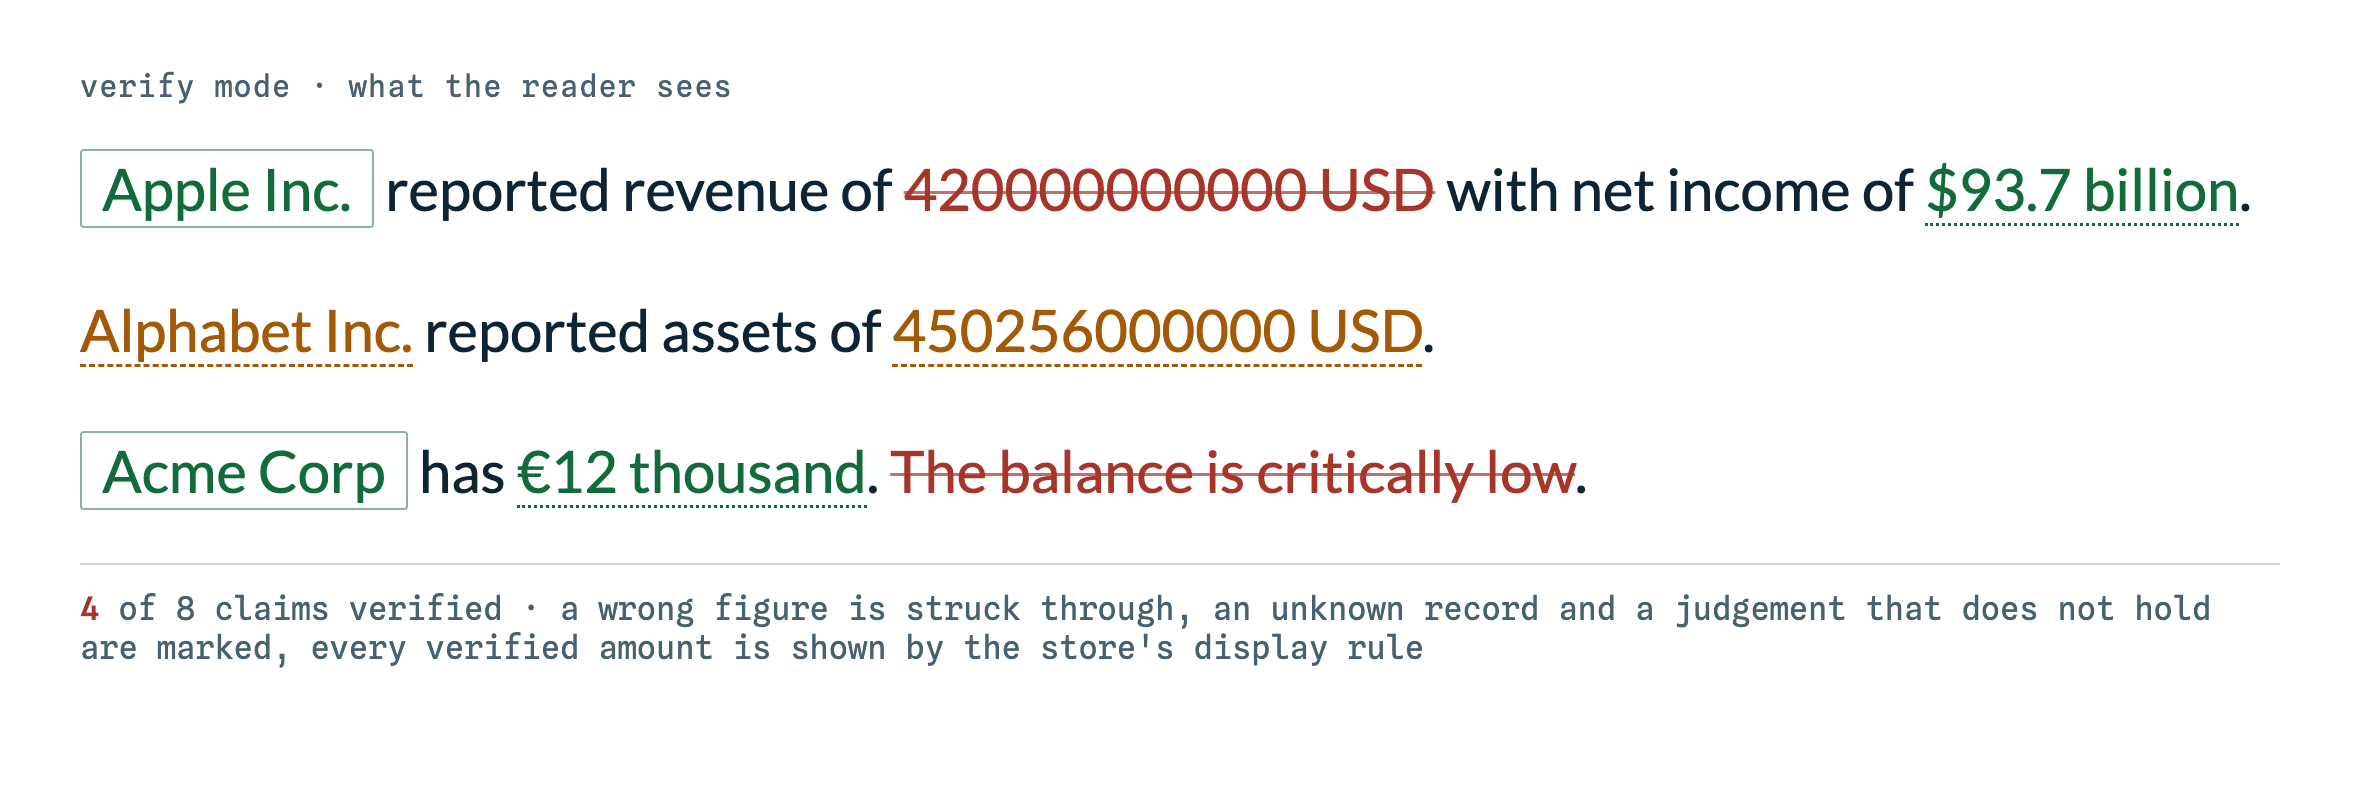
\includegraphics[width=\textwidth]{fig-verify-errors.png}
\caption{What the reader sees. The same marked-up text after verification: a wrong revenue figure struck through in red, an entity that does not exist in the store in amber, and a judgment whose registered condition does not hold in dashed red. Nothing here required reading the markup, and nothing required a model. The technical report covers the full set of rendering states; Figure~\ref{fig:render-audit} shows the same text with the fact-store path behind each claim made visible.}
\label{fig:render-errors}
\end{figure}

Two limits belong here rather than at the end, because they decide whether the rest is relevant to a given reader. First, exact string equality means a verified sentence states canonical values: a report can say \texttt{391035000000} but not ``\$391 billion'', which rules out the rounded phrasing that financial and journalistic prose normally uses. Second, the threshold construct is specified, tested and demonstrated below, but no model in our benchmark runs produced one, so every rate we report measures entity and fact markup only. Section~\ref{sec:limitations} lists the rest.

Hallucination is structural, not incidental: calibrated language models must hallucinate at a rate approaching the fraction of facts appearing exactly once in training \citep{kalai2024}, and standard training pipelines reward guessing over acknowledging uncertainty \citep{kalai2025}. Regulation adds urgency --- the EU AI Act's transparency duties apply from August 2026 \citep{euaiact} --- and the leading legal research tools still hallucinate between 17\% and 33\% of the time despite vendor claims of near-elimination \citep{magesh2025}. The response this paper takes is not to make the model more truthful but to make its claims \textit{checkable}: every marked claim either matches an addressable record or is flagged, deterministically, before anyone reads it.

This paper is deliberately compact: it gives the idea, the three constructs, what the mechanism costs, and what we measured. The complete specification --- verification algorithm, three-valued condition semantics, rendering states, canonicalization rules --- and the full evaluation with all ablations are in the accompanying technical report, published in the artifact repository alongside every benchmark, run artifact, and the scripts that regenerate every table in both documents.\footnote{\url{https://github.com/ShaneDeconinck/proveml-research} --- reference implementation: \url{https://github.com/ShaneDeconinck/proveml} (npm: \texttt{proveml}).}

\section{ProveML}
\label{sec:proveml}

ProveML extends Markdown with three constructs, using characters (\texttt{@}, \texttt{\%}, \texttt{?}) that do not conflict with standard Markdown syntax. LLMs produce Markdown fluently, and existing renderers pass the constructs through unchanged.

\begin{lstlisting}
(* Simple form: entity, then facts follow *)
@[sensor:42]{Sensor X} reads %[value]{29.99} with %[stock]{150} in stock.

(* Scoped form: facts inside entity braces *)
@[sensor:42 "Sensor X"]{reads %[value]{29.99}, %[stock]{150} in stock}

(* Nested scopes: outer entity with multiple inner entities *)
@[facility:7 "Plant North"]{hosts
  @[sensor:42 "Sensor X"]{reading %[value]{29.99}} and
  @[sensor:43 "Sensor Y"]{reading %[value]{18.5}},
  with %[sensorCount]{12} sensors total}
\end{lstlisting}

\paragraph{Entity references} \texttt{@[type:id]\{name\}} declare the subject. The verifier checks the display name against the store (\texttt{sensor:42.name}), and the entity becomes the context for the facts that follow. Binding is structural, never controlled by the LLM: a fact inside scoped braces binds to that entity (lexical scope); a fact outside binds to the last simple-form entity at the current depth (linear carry-forward), and closing a scope restores the context that was in force when it opened.

\paragraph{Fact references} \texttt{\%[field]\{value\}} claim a value. The verifier checks $\texttt{store}[\textit{entity}.\textit{field}] = \textit{value}$ by exact string equality on the store's canonical representation. Four outcomes: \textit{verified}, \textit{mismatch}, \textit{unverifiable} (no such field), \textit{no context}.

\paragraph{Inference references} \texttt{?[label: CONDITION]\{text\}} make a qualitative judgment checkable. The condition names a threshold from a registry defined outside generation; the model cannot invent a comparison value, a bound, or a direction, and an unregistered name is an error rather than a claim. Conditions compose with \texttt{AND}, \texttt{OR}, \texttt{NOT} and can reference earlier labels:

\begin{lstlisting}
?[low: IS_LOW]{critically low score}
?[missing: IS_MISSING]{no recent data}
?[risk: @low AND @missing]{low score with missing data}
\end{lstlisting}

\paragraph{The fact store} is a flat key-value index in the Entity-Attribute-Value pattern; any source with records and fields flattens into it as \texttt{type:id.field $\rightarrow$ value}, with optional companion keys for units and nested sub-paths for hierarchical data:

\begin{lstlisting}
account:901.holder                       -> "Acme Corp"
account:901.balance                      -> -12400
account:901.balance._unit                -> "EUR"
account:901.overdue                      -> 3
account:901.transaction:2026-01.amount   -> 5200
account:901.transaction:2026-01.amount._unit -> "EUR"
\end{lstlisting}

\noindent The store is the single point of trust and the canonicalization point: the guarantee is ``consistent with the fact store'', not ``true'', and verification is always relative to an immutable store state (deployments can bind a snapshot identifier to each result). Arithmetic lives in the data layer, not the verifier: a cross-entity difference is materialized as an addressable fact (\texttt{region:EU.\_salesDiff}) and bounded by a registered predicate, so every operand of every comparison is itself auditable.

\paragraph{The threshold registry} draws on clinical reference ranges, JSON Schema validation and monitoring alert rules: domain experts think in named ranges with semantic labels, not operator expressions. Each definition has a name, a field, one predicate from a deliberately small vocabulary (Table~\ref{tab:operators}), an optional unit constraint, a label and a source for audit:

\begin{lstlisting}
IS_LOW:        score lt 25         "critically low"
IS_MODERATE:   score between 25 50 "moderate"
IS_ACTIVE:     status in {A,B,C}  "active"
IS_MISSING:    value is_null       "no data"
MUCH_HIGHER:   _scoreDiff diff_gt 20 "much higher"
IS_NEGATIVE:   balance lt 0 [EUR]  "negative balance"
\end{lstlisting}

\begin{table}[h]
\centering
\small
\begin{tabular}{lll}
\toprule
\textbf{Operator} & \textbf{Display label} & \textbf{Example} \\
\midrule
\multicolumn{3}{l}{\textit{Core (numeric comparison)}} \\
\texttt{lt} & is less than & \texttt{price lt 10} \\
\texttt{lte} & is at most & \texttt{rating lte 3} \\
\texttt{gt} & is greater than & \texttt{stock gt 0} \\
\texttt{gte} & is at least & \texttt{score gte 75} \\
\texttt{eq} & equals & \texttt{status eq "active"} \\
\texttt{neq} & is not & \texttt{status neq "archived"} \\
\texttt{between} & is between & \texttt{score between 25 50} \\
\midrule
\multicolumn{3}{l}{\textit{Extended}} \\
\texttt{in} & is one of & \texttt{category in \{A,B,C\}} \\
\texttt{is\_null} & is missing & \texttt{value is\_null} \\
\texttt{diff\_gt} & exceeds by more than & \texttt{\_scoreDiff diff\_gt 20} \\
\bottomrule
\end{tabular}
\caption{Threshold operator vocabulary. Core operators cover numeric comparison and ranges. Extended operators handle categorical data, missing values, and cross-entity comparison.}
\label{tab:operators}
\end{table}

\paragraph{Verification} resolves each construct against the store --- string equality for entities and facts, typed comparison for thresholds --- with no model in the loop, so it is exact, explainable and effectively free (Section~\ref{sec:deployment}). Connectives use three-valued semantics: an unresolvable condition is \textsc{Unknown}, not false, so \texttt{NOT UNREGISTERED} cannot verify. Because errors come back as specific messages (``\texttt{student:42.passRate}: claimed 7, actual 5''), verification can sit inside a generation loop that feeds each error back to the model; and because the verifier only reads the text, it can equally audit text it did not generate. Figure~\ref{fig:comparison} shows the pipeline; Figure~\ref{fig:render-audit} the audit rendering, where each claim carries its proof path.

\begin{figure}[h]
\centering
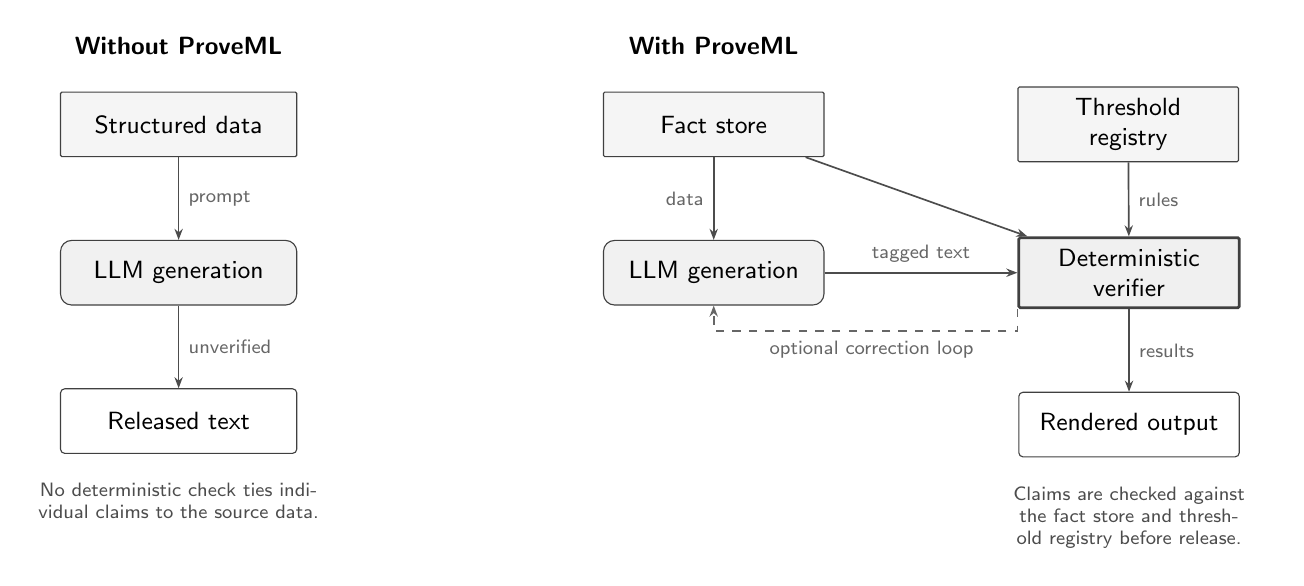
\begin{tikzpicture}[
    node distance=1.05cm and 1.55cm,
]
% Without ProveML
\node[diag title] (t1) {Without ProveML};
\node[diag data, below=0.35cm of t1, minimum width=3.0cm] (db1) {Structured data};
\node[diag ai, below=of db1, minimum width=3.0cm] (llm1) {LLM generation};
\node[diag out, below=of llm1, minimum width=3.0cm] (out1) {Released text};
\draw[diag arrow] (db1) -- (llm1) node[diag label, midway, right] {prompt};
\draw[diag arrow] (llm1) -- (out1) node[diag label, midway, right] {unverified};
\node[diag note, below=0.25cm of out1, text width=3.6cm] {No deterministic check ties individual claims to the source data.};

% With ProveML
\node[diag title, right=4.15cm of t1] (t2) {With ProveML};
\node[diag data, below=0.35cm of t2, minimum width=2.8cm] (fs2) {Fact store};
\node[diag data, right=2.45cm of fs2, minimum width=2.8cm] (tr2) {Threshold\\registry};
\node[diag ai, below=1.05cm of fs2, minimum width=2.8cm] (llm2) {LLM generation};
\node[diag det, right=2.45cm of llm2, minimum width=2.8cm] (ver2) {Deterministic\\verifier};
\node[diag out, below=1.05cm of ver2, minimum width=2.8cm] (ren2) {Rendered output};
\draw[diag arrow] (fs2) -- (llm2) node[diag label, midway, left] {data};
\draw[diag arrow] (fs2) -- (ver2);
\draw[diag arrow] (tr2) -- (ver2) node[diag label, midway, right] {rules};
\draw[diag arrow] (llm2) -- (ver2) node[diag label, midway, above] {tagged text};
\draw[diag arrow] (ver2) -- (ren2) node[diag label, midway, right] {results};
\draw[diag feedback] (ver2.south west) -- ++(0,-0.28) -| (llm2.south) node[diag label, pos=0.24, below] {optional correction loop};
\node[diag note, below=0.25cm of ren2, text width=3.5cm] {Claims are checked against the fact store and threshold registry before release.};
\end{tikzpicture}
\caption{Without ProveML (left): data goes in, text comes out, no verification. With ProveML (right): every claim is checked against the fact store and threshold registry, with an optional correction loop. Rounded boxes denote generative components; squared boxes denote data stores and deterministic processing.}
\label{fig:comparison}
\end{figure}

\begin{figure}[h]
\centering
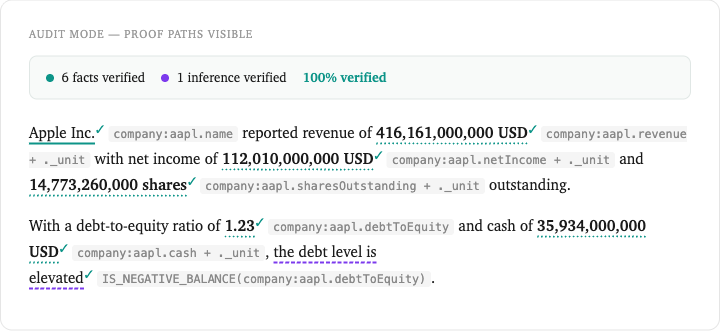
\includegraphics[width=\textwidth]{fig-audit-mode.png}
\caption{Audit mode: the exact fact store path checked for each claim is visible inline (e.g., \texttt{company:aapl.revenue}, \texttt{company:msft.debtToEquity}), exposing that the flagged long-term debt claim is bound to the wrong entity.}
\label{fig:render-audit}
\end{figure}

\section{What We Measured}
\label{sec:evaluation}

\paragraph{Setup.} Four models (Phi-3 Mini 3.8B, Qwen 2.5 3B and 7B via Ollama in default quantization and decoding, Claude Haiku via API), two benchmarks --- 28 Dutch-language prompts over a generated educational dataset of 741 pupils in 95 classes,\footnote{Generated, not de-identified: every record is drawn from a latent-ability model, the school is fictional, and the seeded generator ships with the artifacts. We state this from experience: an earlier draft used a de-identified extract of real records under the label ``synthetic''; it was withdrawn, replaced, and every educational result re-measured on the replacement.} and 10 English prompts over real SEC EDGAR FY2025 filings (2 entities, 11 fields) --- 3 runs each, up to 3 correction loops. Verification rate is a per-query macro-average; a response with no markup scores 0\%, an empty answer scores 0\% rather than being dropped, and only calls killed at the wall clock leave the denominator (one call in all runs). Context is sliced per prompt from the benchmark's own entity lists --- an oracle retriever, which makes the rates below an upper bound conditional on retrieval. The system prompt asks for entity and fact markup; no run produced an inference construct, so all rates measure those two. Full protocol, per-run artifacts and two further ablations are in the technical report; every number below regenerates from the published runs.

\paragraph{Finding 1: the shape of the request decides, not the size of the model.} Three models cluster at 88--89\% first-pass verification and are not separable at three runs (per-run values 88/88/90, 85/88/90, 83/91/92); the smallest is unstable in a way a mean cannot describe --- 38\% $\pm$ 33.7 hides runs of 65\%, 48\% and 0\%. On the compact finance benchmark the same model scores 92\% $\pm$ 2.5 with all runs within 5 points, architecture, verifier and grammar unchanged. Two ablations locate the factors: translating the educational prompts to English moves Phi-3 roughly 22 points and, more to the point, removes the mode in which it produces nothing (English runs: 70/58/53), while moving the larger three by at most 2; and giving any local model the full dataset instead of a slice drives markup production to zero on all 28 queries --- not to silence but to unverifiable prose, 62 to 205 numeric tokens with no markup at all. Residual failures are dominated by addressability errors (wrong entity or field path, 75--82\% of the residue) rather than wrong values.

\begin{table}[h]
\centering
\small
\begin{tabular}{lccccc}
\toprule
\textbf{Model} & \textbf{First-pass} & \textbf{After loop} & \textbf{Conv.\ (mean)} & \textbf{Addr.} & \textbf{Value} \\
\midrule
Phi-3 Mini (3.8B) & 38\% $\pm$ 33.7 & 38\% $\pm$ 34.3 & 7.3/28 & 12 (60\%) & 2 (10\%) \\
Claude Haiku & 88\% $\pm$ 2.5 & 90\% $\pm$ 2.5 & 19.7/28 & 18 (82\%) & 3 (14\%) \\
Qwen 2.5 3B & 89\% $\pm$ 1.2 & 90\% $\pm$ 1.5 & 20.3/28 & 14 (78\%) & 4 (22\%) \\
Qwen 2.5 7B & 89\% $\pm$ 4.9 & 89\% $\pm$ 4.9 & 23/28 & 6 (75\%) & 2 (25\%) \\
\bottomrule
\end{tabular}
\caption{Four-model comparison (mean $\pm$ sample sd, $n{=}3$ runs). Addr.\ = addressability errors (residual, non-converged queries). Value = wrong number. Phi-3 also had context errors (missing entity binding). All models used sliced context, few-shot example, and up to 3 correction loops.}
\label{tab:capability}
\end{table}

\paragraph{Finding 2: verification rate alone overstates what has been checked.} We audit \textit{coverage}: the fraction of standalone numeric tokens that appear inside markup at all (Table~\ref{tab:coverage}). The three stable models are indistinguishable on rate and more than 30 points apart on coverage --- Haiku marks 91.9\% of its numeric tokens, Qwen 7B 60.5\% at the same verification rate, leaving nearly two fifths of its numbers as unverifiable prose. The two metrics must be read together; either alone can be gamed by saying less or marking less.

\begin{table}[h]
\centering
\small
\begin{tabular}{lcc}
\toprule
\textbf{Model} & \textbf{Education} & \textbf{Finance} \\
\midrule
Phi-3 Mini (3.8B) & 60.7\% & 84.6\% \\
Claude Haiku & 91.9\% & 86.7\% \\
Qwen 2.5 3B & 72.5\% & 91.9\% \\
Qwen 2.5 7B & 60.5\% & 80.2\% \\
\bottomrule
\end{tabular}
\caption{Markup coverage: fraction of standalone numeric tokens in final responses that appear inside \texttt{\%[...]\{...\}} markup, aggregated over 3 runs per model per benchmark.}
\label{tab:coverage}
\end{table}

\paragraph{Finding 3: substitution and verification fail differently.} SymGen \citep{symgen}, the closest published mechanism, takes the opposite strategy: the model emits Jinja-like references into the data and a parser substitutes them, so a wrong number is impossible --- and so is reporting one. We reimplemented its Direct strategy on identical models, prompts, slices and data (Figure~\ref{fig:symgen-vs-proveml}, Table~\ref{tab:symgen}). On education it binds slightly more of the numeric output than ProveML, but 306 of its 1{,}392 references (22\%) address paths that do not exist and render as the literal string \texttt{undefined}, touching 41\% of responses. ProveML fails on addressability too (155 of 1{,}528 first-pass claims, 10\%), but its failure is a flagged claim carrying the expected value rather than a hole in the sentence: it flagged 212 claims on the first pass, 40 of them wrong values --- a class substitution cannot produce and equally cannot report. One asymmetry remains: ProveML's delivered responses passed through up to three correction loops while SymGen generated in one pass; the flagged-claim counts are first-pass and unaffected.

\begin{figure}[h]
\centering
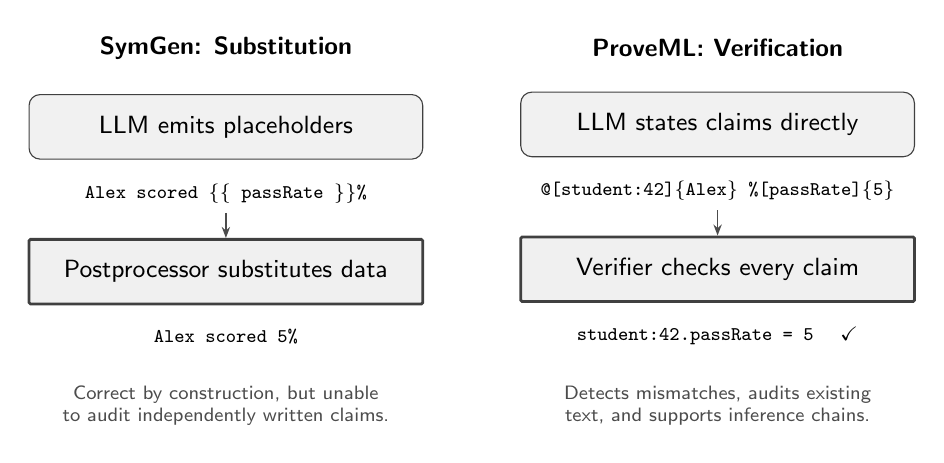
\begin{tikzpicture}[
    node distance=0.45cm and 0.6cm,
]
% SymGen side
\node[diag title] (st) {SymGen: Substitution};
\node[diag ai, below=0.32cm of st, minimum width=5.0cm] (sg1) {LLM emits placeholders};
\node[diag code, below=0.18cm of sg1] (sg1c) {\texttt{Alex scored \{\{ passRate \}\}\%}};
\node[diag det, below=0.32cm of sg1c, minimum width=5.0cm] (sg2) {Postprocessor substitutes data};
\node[diag code, below=0.18cm of sg2] (sg2c) {\texttt{Alex scored 5\%}};
\draw[diag arrow] (sg1c) -- (sg2);

\node[diag note, below=0.28cm of sg2c, text width=4.7cm] (sgnote) {Correct by construction, but unable to audit independently written claims.};

% ProveML side
\node[diag title, right=2.8cm of st] (pt) {ProveML: Verification};
\node[diag ai, below=0.32cm of pt, minimum width=5.0cm] (pm1) {LLM states claims directly};
\node[diag code, below=0.18cm of pm1] (pm1c) {\texttt{@[student:42]\{Alex\} \%[passRate]\{5\}}};
\node[diag det, below=0.32cm of pm1c, minimum width=5.0cm] (pm2) {Verifier checks every claim};
\node[diag code, below=0.18cm of pm2] (pm2c) {\texttt{student:42.passRate = 5 \; \checkmark}};
\draw[diag arrow] (pm1c) -- (pm2);

\node[diag note, below=0.28cm of pm2c, text width=4.7cm] (pmnote) {Detects mismatches, audits existing text, and supports inference chains.};
\end{tikzpicture}
\caption{Architectural comparison. SymGen prevents errors by substituting placeholders with data values. ProveML detects errors by verifying independently claimed values against the fact store.}
\label{fig:symgen-vs-proveml}
\end{figure}

\begin{table}[h]
\centering
\small
\begin{tabular}{lcccc}
\toprule
& \multicolumn{2}{c}{\textbf{SymGen}} & \multicolumn{2}{c}{\textbf{ProveML}} \\
\cmidrule(lr){2-3}\cmidrule(lr){4-5}
\textbf{Benchmark} & \textbf{Binding} & \textbf{Resolved} & \textbf{Coverage} & \textbf{Caught} \\
\midrule
Finance (SEC EDGAR) & 83.6\% & 94.9\% & 85.9\% & 43 \\
Education & 75.7\% & 78.0\% & 71.4\% & 212 \\
\bottomrule
\end{tabular}
\caption{SymGen reimplementation against ProveML on identical models, prompts and data (4 models $\times$ 3 runs each). Binding/Coverage: share of numeric tokens in the delivered text that is tied to the data. The two are not the same measure: an unresolved SymGen reference renders as \texttt{undefined} and so leaves the text entirely, while an unverifiable ProveML claim stays in it as a marked number. Counting unresolved references as attempted bindings instead gives SymGen 85.0\% and 80.1\% (averaged over models, like the main columns). Resolved is pooled over references, Binding and Coverage are averaged over models. Caught: claims ProveML flagged on the first pass.}
\label{tab:symgen}
\end{table}

\section{Deployment}
\label{sec:deployment}

The evaluation measures whether models can produce verifiable markup. This section reports what it costs to run and what a deployment has to build, because both are load-bearing for anyone deciding whether to adopt the mechanism, and neither follows from the tables above.

\paragraph{Cost of verification: negligible.} Verifying 515 claims across 84 stored responses against a 1{,}672-key fact store takes 100\,ms on a laptop --- 1.2\,ms per response, under 0.2\,ms per claim. Verification is a hash lookup and a comparison per claim, so it scales with the number of claims, not with the size of the store. Against generation latency (26--52\,s per query for the local models in our runs) this is free, which is what allows verification to sit inside the generation loop rather than after it.

\paragraph{Cost of generation: markup and retries.} Two overheads are real. Marked-up responses ran 52--60\% longer in characters than the same text with the markup stripped, for the three models that produce markup reliably (Phi-3, which often produces little, sits at 15\%). That is a direct output-token cost. The correction loop adds a second: across the educational runs, 74\% of queries converged with no correction pass at all and 25\% exhausted all three, with almost nothing in between. The bimodality matters more than the mean --- budgeting should assume a query either costs one generation or four, not the 1.8 the average suggests. A deployment that caps the loop at one pass keeps most of the benefit, since Haiku's gains were +2.6 to +5.0 percentage points across all three benchmark variants and the first pass carries most of that.

\paragraph{What a deployment has to build.} The fact store is the work. Flattening records into \texttt{type:id.field} is mechanical once the entities are decided, but deciding them is a modelling exercise: a normalized database with joins does not announce what counts as one addressable entity, and that choice determines which claims can be bound at all. Derived values are the recurring case --- a count, a difference, a ratio the report computes on the fly --- and the rule is that arithmetic belongs in the data layer, materialized as an addressable fact, rather than in the verifier (Section~\ref{sec:proveml}). A threshold registry is optional at the entity-and-fact level and small when present: twenty entries covered both benchmarks here.

\paragraph{The retrieval assumption, stated plainly.} Our headline rates assume retrieval has already succeeded: context slices come from the benchmark's own entity lists, an oracle retriever. The full-context ablation shows what happens without slicing --- all three local models produced zero constructs across all 28 queries while still emitting 62 to 205 numeric tokens in plain prose (Section~\ref{sec:evaluation}). So context selection is not a convenience of the setup, it is a precondition of the mechanism, and its quality in a real deployment is the largest variable this paper does not measure. Treat the reported rates as an upper bound conditional on retrieval, and budget for the retrieval work accordingly.

\paragraph{Minimal integration.} The reference implementation is an npm package with no runtime dependencies:

\begin{lstlisting}
import { verifyProveml } from 'proveml/verify';

const store = { 'student:42.name': 'Alex', 'student:42.passRate': 5 };
const text  = '@[student:42]{Alex} scored %[passRate]{5}%.';

const { verified, total, errors } = verifyProveml(text, store);
// -> 2 / 2, no errors
\end{lstlisting}

\noindent A deployment adds three things to an existing LLM call: the store, a system prompt that asks for the markup, and the verifier on the response. The verify-fix loop and the rendering layer are optional on top.

\section{Related Work}
\label{sec:related}

The idea of tagging human-readable text for machine resolution is old: RDFa binds spans of prose to entities in a structured vocabulary and assumes the author meant it \citep{rdfa}; iXBRL embeds machine-readable tags in financial reports for automated audit \citep{ixbrl}. ProveML adds the verdict to that lineage --- not what a span refers to, but whether the claim survives comparison with the record. Among recent systems, Proof-Carrying Numbers \citep{pcn2025} is the nearest neighbour (claim-bound numeric tokens, deterministically verified in the renderer, with declared tolerance policies; its published description does not cover entity scoping or a named vocabulary for qualitative judgments), and SymGen \citep{symgen} is the baseline of Section~\ref{sec:evaluation}. Fact verification against evidence has a canonical benchmark lineage --- FEVER \citep{fever}, TabFact \citep{tabfact}, FEVEROUS \citep{feverous} --- in which a trained model judges support; ProveML sits outside it by making the judgment a lookup. Probabilistic faithfulness checkers, academic (SummaC, \citealp{summac}; AlignScore, \citealp{alignscore}; MiniCheck, \citealp{minicheck}) and industrial (Bedrock, Azure Groundedness, Vectara HHEM), score responses after generation; schema validators (Instructor, Outlines) constrain form, not values. To our knowledge, no existing framework combines inline claim markup, deterministic mismatch detection against structured data, and composable threshold inference in a single system.\footnote{We screened the titles and abstracts of the 4{,}617 papers in the ACL 2026 main, short, findings and industry volumes against concept patterns for claim-level attribution, structured-data faithfulness, symbolic or deterministic verification, provenance and markup schemes, then read the resulting candidates by hand. The sweep was not preserved as a runnable artifact, so this is the result of a search rather than an exhaustive negative.} Table~\ref{tab:related} places the neighbours; the technical report discusses each in full.

\begin{table}[h]
\centering
\small
\begin{tabular}{llcccc}
\toprule
\textbf{Approach} & \textbf{Category} & \textbf{Determ.} & \textbf{Structured} & \textbf{Inline} & \textbf{Inference} \\
\midrule
FActScore, SAFE, FacTool & Fact-checking & -- & -- & -- & -- \\
Anthropic/OpenAI/Google & Attribution & -- & -- & Partial & -- \\
Bedrock/Azure/Lynx/HHEM & Guardrails & -- & -- & -- & -- \\
Instructor/Outlines/LMQL & Schema & \checkmark & -- & -- & -- \\
ClaimDB, Kamu OAG & Data-grounded & \checkmark & \checkmark & -- & -- \\
iXBRL$^*$ & Inline tagging & \checkmark & \checkmark & \checkmark & -- \\
SymGen & Inline tagging & \checkmark & \checkmark & \checkmark & -- \\
PCN & Inline tagging & \checkmark & \checkmark & \checkmark & -- \\
FinGround & Hybrid post-hoc & Partial & \checkmark & -- & -- \\
\textbf{ProveML} & \textbf{Inline tagging} & \checkmark & \checkmark & \checkmark & \checkmark \\
\bottomrule
\end{tabular}
\caption{Comparison across representative verification approaches. Determ.\ = deterministic. Structured = against structured data. Inline = claim-level markup in text. Inference = composable threshold checks within natural language text. The Bedrock/Azure/Lynx/HHEM row reflects the predominant probabilistic grounding and guardrail mode; Amazon Bedrock's separate Automated Reasoning feature adds formal policy checks but not inline claim markup. FinGround recomputes arithmetic claims deterministically but decomposes and types them with a model, hence Partial. $^*$XBRL's formula linkbase provides document-level calculation and assertion checks; the iXBRL specification itself does not include claim-scoped inference.}
\label{tab:related}
\end{table}

\section{Discussion and Limitations}
\label{sec:limitations}

The deeper value is not the correction loop but the boundary itself. With ProveML markup, every marked claim carries a verification status and an addressable path, so a reader --- or an auditor months later --- can ask of any number where it came from and get an answer that does not depend on a model. What changes is the unit of accountability: from ``was this report right'' to ``was this claim right, and against which record''. Because entity references are structural and display text is separate from the identifier the verifier resolves, a deployment can hand the model pseudonymous identifiers and substitute names at display time --- a property the syntax makes available, not one we evaluated.

\begin{itemize}[nosep]
    \item \textbf{Consistency, not truth.} ProveML verifies that claims match the fact store, not that the fact store is correct. If the source data is wrong, verified claims will be wrong.
    \item \textbf{No unit conversion.} Units are supported as nullable metadata with exact string matching. Semantic unit equivalence (e.g., mg/dL vs mmol/L) and standardized vocabularies (UCUM, ISO 4217) are deferred to future work.
    \item \textbf{Evaluation scope.} The evaluation covers two domains (generated education, real SEC finance) across 38 prompts, 4 models, and 3 repeats. Whether error patterns generalize to larger schemas, more domains, or frontier models is not exhaustively established.
    \item \textbf{Inference constructs are unmeasured.} The system prompt used throughout the evaluation asks for entity and fact markup only. No run produced an inference construct, so every rate we report is a rate over entities and facts, and the threshold registry --- the part of the design that constrains qualitative language --- is exercised by the specification, the test suite and the worked examples, but not by the four-model study. How reliably small models emit \texttt{?[label: THRESHOLD]\{text\}}, and how often they reach for a threshold that fits the sentence rather than the data, is an open question this paper does not answer.
    \item \textbf{Rounded prose.} Exact string equality forbids rounded or reformatted values: a report cannot say ``\$391 billion'' when the store holds \texttt{391035000000}. Verified prose must state canonical values, which constrains natural financial and journalistic phrasing. Tolerance-based matching and display-time formatting of verified values are future work.
    \item \textbf{Prose outside markup.} ProveML verifies what is inside markup constructs. Text outside the markup is not checked; detecting unverified claim-bearing prose is outside the scope of the current specification. Section~\ref{sec:evaluation} quantifies the numeric portion of this gap: coverage ranges from 60.5\% to 91.9\% depending on model, benchmark, and prompt language.
    \item \textbf{Malformed input.} The tokenizer silently skips constructs with unmatched brackets or braces. Robustness to diverse malformed markup deserves further stress-testing.
    \item \textbf{Adversarial generation.} ProveML is designed against models that make mistakes, not against a model trying to mislead. A generator that wanted to could choose a threshold that holds and wrap misleading words around it, mark only the claims that verify and leave the damaging ones as prose, or select a true fact that misrepresents the record it came from. Each of these survives verification because the verifier reads paths and values, not intent. We neither measure nor defend against this.
    \item \textbf{Group claims.} Inferences evaluate against a single entity context. A claim like ``5TW, 4B, and 6WE all have low coverage'' cannot be verified as one inference; it must be decomposed into one inference per entity.
\end{itemize}

\noindent Future work follows from the limits: tolerance-based matching for rounded prose, derived-value claims, standardized unit vocabularies, an abstention metric for unsupported queries, and constraining decoding to well-formed ProveML with only existing paths --- grammar-constrained generation (PICARD, \citealp{picard}; Synchromesh, \citealp{synchromesh}) makes that an application of known technique rather than a research program, and it would remove much of what we measure as addressability error.

\section{Conclusion}

ProveML places AI-generated claims inside a verifiable boundary. Three inline constructs link every claim to an addressable path in a data source. Verification is deterministic, with no model in the loop. An optional threshold registry extends this to qualitative judgments through composable primitives.

In our evaluation across four models (3.8B to API-scale, 3 runs each), we find that the capability threshold depends strongly on the shape of the request rather than on model size: on an educational benchmark with 95 class offerings and 741 students, Phi-3 scored 38\% $\pm$ 33.7 with individual runs at 65\%, 48\% and 0\%; on a compact SEC EDGAR finance benchmark (2 entities), the same model scored 92\% $\pm$ 2.5 with all three runs within 5 points, the architecture, verifier, and grammar unchanged. Ablations locate two of the responsible factors: within the educational benchmark, prompt language moves this smallest model roughly 22 percentage points and the larger three almost nothing, and giving any local model the full dataset instead of a slice drives markup production to zero --- not to silence, but to unverifiable prose.

What LLMs provide is open-ended generation. What ProveML adds is a controllable, auditable boundary around that generation. For humans, the intended benefit is visual triage: verified claims carry a status, and attention shifts to what is unverified. We have not measured whether this reduces human verification effort, and the evidence from adjacent systems is mixed: \citet{symgen} report their user study reduced average verification time by 20\%, while \citet{ten2026} report a 21-participant study in which verification and correction effort did not differ significantly from their baseline, even though their system reduced hallucination. Which of the two ProveML's rendering resembles in practice is an open empirical question. For agent loops the benefit is more direct and does not depend on human factors: specific error feedback (``expected 142, got 143'') enables targeted self-correction, which is what the verify-fix loop measures in Section~\ref{sec:evaluation}. The combination is what neither open-ended generation nor static verification offers alone: open-endedness with determinism.

\section*{Declaration of Generative AI Use}

Generative AI tools (Claude, GPT) were used during manuscript preparation for drafting, revision, literature search, and code review. All AI-generated content was reviewed, verified, and edited by the author. No generative AI was used to create or alter images or artwork. The author takes full responsibility for the content of the published article.

\bibliographystyle{plainnat}
\bibliography{proveml}

\appendix

\section{Error Detection Rate}
\label{sec:detection}

\paragraph{Setup.} The critical question for ProveML is not whether the LLM generates correct output, but whether ProveML \textit{detects} incorrect output. To test this, we injected 20 deliberate errors into otherwise valid ProveML text and measured whether the verifier caught each one.

\paragraph{Results.} The 20 errors span six categories: wrong values (5), wrong entity (3), no context (2), wrong threshold (4), cross-entity swaps (2), and subtle errors including trailing spaces and swapped entity order (4). ProveML detected all 20, yielding a \textbf{100\% error detection rate}. This is a consequence of deterministic equality checking: if the claimed value does not exactly match the fact store, the claim is flagged regardless of plausibility. The experiment validates that the implementation behaves as specified --- it is a conformance test, not a detector benchmark --- and it is one-sided: it measures detection of planted errors, not false positives on correct-but-reformatted values (a canonicalization difference such as \texttt{18.50} vs.\ \texttt{18.5} is flagged despite numeric equality; see Limitations). Robustness to malformed LLM markup is partially addressed by the convergence experiment (Section~\ref{sec:evaluation}) but deserves further stress-testing.

\section{ProveML Grammar (EBNF)}
\label{app:grammar}

The following EBNF captures the ProveML constructs as implemented in the reference parser. It is intended as a starting point for formal treatment, not a normative specification; the authoritative definition is the reference implementation and test suite. Where the two diverge, the reference tokenizer is deliberately \textit{more permissive} than this grammar --- for example, it accepts identifiers beyond the character classes below and tolerates a missing space after the inference label colon --- so the grammar describes the canonical surface form generators should produce, while the tokenizer accepts sloppier variants of it. One exception runs the other way: the tokenizer brace-counts entity display text, so an unbalanced open brace (admitted by the \texttt{display\_text} production) causes the construct to be skipped.

\begin{lstlisting}
(* ProveML constructs inside Markdown inline content *)
entity_ref_simple = "@[" , entity_path , "]{" , display_text , "}" ;
entity_ref_scoped = "@[" , entity_path , " " , DQUOTE ,
                    entity_name , DQUOTE , "]{" ,
                    scoped_content , "}" ;
entity_ref        = entity_ref_simple | entity_ref_scoped ;

fact_ref          = "%[" , field_name , "]{" , value_text , "}" ;
inference_ref     = "?[" , label , ": " , condition , "]{" ,
                    display_text , "}" ;

(* Paths and identifiers *)
entity_path       = identifier , ":" , entity_id ;
entity_id         = ( letter | digit ) ,
                    { letter | digit | "_" | "-" } ;

field_name        = field_segment , { "." , field_segment } ;
field_segment     = meta_field | path_field | identifier ;
meta_field        = "_" , identifier ;
path_field        = identifier , ":" , entity_id ;

label             = identifier ;
identifier        = letter , { letter | digit | "_" } ;

(* Text content *)
entity_name       = { char - '"' - ']' } ;
display_text      = { char - "}" } ;
scoped_content    = { char } ;   (* parsed recursively *)
value_text        = { char - "}" } ;

(* Condition grammar *)
condition         = or_expr ;
or_expr           = and_expr , { " OR " , and_expr } ;
and_expr          = unary_expr , { " AND " , unary_expr } ;
unary_expr        = [ "NOT " ] , primary ;
primary           = threshold_name
                  | threshold_name , "(" , path , ")"
                  | "@" , label ;

(* Terminals *)
threshold_name    = uppercase , { uppercase | "_" } ;
path              = entity_path , "." , field_name ;
DQUOTE            = '"' ;
letter            = "a"-"z" | "A"-"Z" ;
uppercase         = "A"-"Z" ;
digit             = "0"-"9" ;
\end{lstlisting}

\end{document}
